\chapter{Caracterización Experimental del Transistor MOSFET 2N7000}
\label{chap:caracterizacion_mosfet}

A diferencia de los transistores bipolares, en los cuales la tensión base-emisor en conducción activa directa puede
estimarse razonablemente en $V_{BE} \approx 0.65\V \text{ a } 0.70\V$, los transistores MOSFET de enriquecimiento
presentan una marcada dispersión de fabricación en sus parámetros electrofísicos fundamentales. De acuerdo con la
hoja de datos del fabricante ON Semiconductor para el modelo 2N7000, la tensión umbral de conducción ($V_{th}$) puede
oscilar entre $0.8\V$ y $3.0\V$. Por ende, la formulación de un diseño analítico riguroso exige la previa caracterización
experimental del ejemplar específico a emplear en el laboratorio.

\section{Fundamento Teórico y Modelo Cuadrático de Saturación}

Para un MOSFET de canal N tipo enriquecimiento que opera en la región de saturación (también denominada zona activa o de
corriente constante), la tensión drenador-surtidor satisface la condición $V_{DS} \ge V_{GS} - V_{th}$, formándose un
estrangulamiento del canal (\textit{pinch-off}) en el extremo contiguo al drenador. En tales condiciones, la corriente de
drenador ($I_D$) queda gobernada por la ecuación cuadrática de Shockley para transistores de efecto de campo:
\begin{equation}
  I_D = \frac{K}{2} \cdot (V_{GS} - V_{th})^2
  \label{eq:shockley_mosfet}
\end{equation}
donde $K$ es el parámetro de transconductancia del transistor (en $\mA/\V^2$ o $\A/\V^2$) y $V_{th}$ es la tensión
umbral (\textit{threshold voltage}), a partir de la cual se induce el canal conductor de electrones bajo el óxido de compuerta.

Para extraer de manera precisa estos dos parámetros intrínsecos a partir de pares coordenados $(V_{GS}, I_D)$ medidos
experimentalmente, se aplica la raíz cuadrada a ambos miembros de la ecuación~\eqref{eq:shockley_mosfet}:
\begin{equation}
  \sqrt{I_D} = \sqrt{\frac{K}{2}} \cdot (V_{GS} - V_{th}) = m \cdot V_{GS} + b
  \label{eq:recta_raiz_id}
\end{equation}

La expresión obtenida corresponde a una función lineal $y = m \cdot x + b$, donde la variable independiente es
$x = V_{GS}$ y la variable dependiente es $y = \sqrt{I_D}$. La pendiente $m$ y la ordenada al origen $b$ se vinculan
directamente con los parámetros del modelo según:
\begin{equation}
  m = \sqrt{\frac{K}{2}} \implies K = 2 \cdot m^2
  \label{eq:parametro_K}
\end{equation}
\begin{equation}
  b = -m \cdot V_{th} \implies V_{th} = -\frac{b}{m} = \frac{|b|}{m}
  \label{eq:parametro_Vth}
\end{equation}

\section{Montaje Experimental y Registro de Mediciones}

Para relevar los puntos de la curva de transferencia, se polarizó el transistor 2N7000 disponiendo un resistor de carga
de drenador $R_D = 10.1\kohm$ y aplicando una tensión variable de compuerta mediante una fuente regulada con ajuste fino.
Se verificó en cada punto que la tensión drenador-surtidor excediera holgadamente el margen de saturación
($V_{DS} > V_{GS} - V_{th}$), asegurando que el dispositivo operase en régimen cuadrático estricto.

En el Cuadro~\ref{tab:mediciones_2n7000} se transcriben las mediciones de tensión $V_{GS}$, la corriente de drenador
$I_D$ relevada y los valores calculados de $\sqrt{I_D}$ (correspondientes al archivo de cálculo \texttt{2n7000.ods}).

\begin{table}[!ht]
  \centering
  \begin{tabular}{|c|c|c|c|}
    \hline
    \textbf{Medición N°} & $V_{GS}\ [\V]$ & $I_D\ [\mA]$ & $\sqrt{I_D}\ [\mathrm{A}^{1/2}]$ \\
    \hline
    1 & $1.751$ & $0.62$ & $0.02490$ \\
    2 & $1.777$ & $0.82$ & $0.02864$ \\
    3 & $1.798$ & $1.03$ & $0.03209$ \\
    4 & $1.812$ & $1.19$ & $0.03450$ \\
    5 & $1.826$ & $1.39$ & $0.03728$ \\
    \hline
  \end{tabular}
  \caption{Puntos experimentales relevados para la caracterización del MOSFET 2N7000 en saturación.}
  \label{tab:mediciones_2n7000}
\end{table}

\section{Regresión Lineal y Extracción de Parámetros}

Aplicando el método de mínimos cuadrados a los pares coordenados $(V_{GS}, \sqrt{I_D})$ del Cuadro~\ref{tab:mediciones_2n7000},
se obtuvieron los siguientes coeficientes estadísticos:
\begin{equation}
  m = 0.164172\ \frac{\mathrm{A}^{1/2}}{\V} = 5.1916\ \frac{\mathrm{mA}^{1/2}}{\V}
\end{equation}
\begin{equation}
  b = -0.262846\ \mathrm{A}^{1/2} = -8.3121\ \mathrm{mA}^{1/2}
\end{equation}
con un coeficiente de determinación $R^2 > 0.999$, lo cual confirma la óptima linealidad cuadrática del dispositivo.

Sustituyendo estos resultados en las ecuaciones~\eqref{eq:parametro_K} y \eqref{eq:parametro_Vth}:
\begin{equation}
  V_{th} = \frac{0.262846\ \mathrm{A}^{1/2}}{0.164172\ \mathrm{A}^{1/2}/\V} \approx 1.60104\V
  \label{eq:Vth_calculado}
\end{equation}
\begin{equation}
  K = 2 \cdot (0.164172\ \mathrm{A}^{1/2}/\V)^2 = 0.053905\ \frac{\A}{\V^2} = 53.905\ \frac{\mA}{\V^2}
  \label{eq:K_calculado}
\end{equation}

En la figura~\ref{fig:plot_caracterizacion} se exhibe el gráfico de la recta ajustada superpuesta a los puntos
experimentales relevados, indicando la extrapolación hacia $\sqrt{I_D} = 0$, donde se localiza la tensión umbral $V_{th}$.

\begin{figure}[!ht]
  \centering
  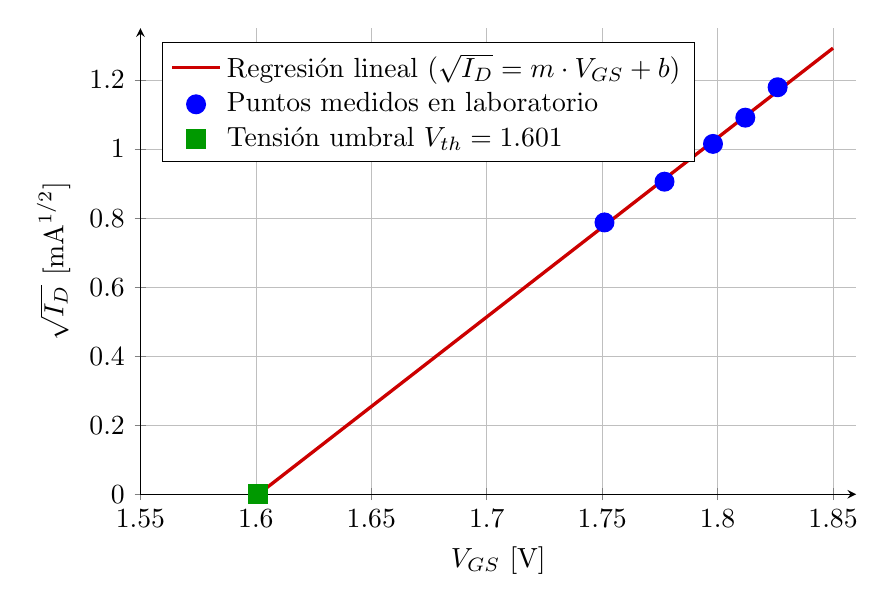
\begin{tikzpicture}
  \begin{axis}[
    width=0.88\textwidth,
    height=7.5cm,
    xlabel={$V_{GS}\ [\mathrm{V}]$},
    ylabel={$\sqrt{I_D}\ [\mathrm{mA}^{1/2}]$},
    xmin=1.55, xmax=1.86,
    ymin=0, ymax=1.35,
    grid=both,
    grid style={line width=.1pt, draw=gray!30},
    major grid style={line width=.2pt, draw=gray!50},
    axis lines=left,
    legend pos=north west,
    legend cell align={left},
    every axis plot/.append style={very thick}
  ]
    % Recta de regresion lineal: y = 5.1916 * x - 8.3121
    \addplot[domain=1.60104:1.85, color=red!80!black, samples=2] {5.1916*x - 8.3121};
    \addlegendentry{Regresión lineal ($\sqrt{I_D} = m \cdot V_{GS} + b$)}

    % Puntos medidos en laboratorio (Hoja 2)
    \addplot[only marks, mark=*, mark size=3pt, color=blue] coordinates {
      (1.751, 0.7874)
      (1.777, 0.9055)
      (1.798, 1.0149)
      (1.812, 1.0909)
      (1.826, 1.1790)
    };
    \addlegendentry{Puntos medidos en laboratorio}

    % Marcador del Vth en y = 0
    \addplot[only marks, mark=square*, mark size=3pt, color=green!60!black] coordinates {
      (1.60104, 0.0)
    };
    \addlegendentry{Tensión umbral $V_{th} = 1.601\V$}

  \end{axis}
\end{tikzpicture}

  \caption{Curva de transferencia linealizada ($\sqrt{I_D}$ en función de $V_{GS}$) y extracción de $V_{th}$ y $K$.}
  \label{fig:plot_caracterizacion}
\end{figure}

Los valores obtenidos ($V_{th} = 1.60104\V$ y $K = 53.905\mA/\V^2$) concuerdan plenamente con las especificaciones
típicas del 2N7000 provistas en su hoja de datos y serán adoptados a lo largo de todos los cálculos de diseño analítico
y modelos de simulación SPICE del presente informe.
